\section{Technik und Territorium: Was Infrastrukturen leisten}

\subsection{Einführung: Infrastruktur als technikgeschichtliches Problem}

Die Vorlesung untersucht,
welche Rolle Infrastrukturen für moderne Gesellschaften spielen.

Im Zentrum steht die Frage,
wie technische Netze,
Verkehrssysteme,
Versorgungssysteme
und digitale Infrastrukturen
Räume erschliessen,
Macht organisieren
und gesellschaftlichen Alltag prägen.

Infrastrukturen sind dabei nicht nur technische Einrichtungen.

Sie sind auch politische,
soziale,
ökonomische
und territoriale Ordnungen.

Sie legen fest,
wer Zugang zu bestimmten Räumen,
Ressourcen
und Möglichkeiten erhält.

Zentrale Leitfragen:

\begin{itemize}
\item Was sind Infrastrukturen?
\item Wie erschliessen Infrastrukturen Territorien?
\item Welche Rolle spielen sie für Macht und Herrschaft?
\item Wie prägen Infrastrukturen Alltag und gesellschaftliche Normalität?
\item Worauf baut die digitale Welt materiell und territorial auf?
\end{itemize}

Die Geschichte der Infrastruktur ist daher
nicht nur eine Geschichte von Brücken,
Strassen,
Kanälen,
Eisenbahnen
oder Rechenzentren.

Sie ist auch eine Geschichte davon,
wie Gesellschaften räumlich,
politisch
und technisch geordnet werden.

\subsection{Nachtrag: Umwelt als gesellschaftspolitisches Thema}

Zu Beginn der Sitzung wurde nochmals
an die vorherige Vorlesung
zu Umweltkatastrophen und Umweltbewusstsein angeknüpft.

Umwelt entstand als gesellschaftspolitisches Thema
seit den 1960er Jahren
aus einer Kombination verschiedener Entwicklungen.

Dazu gehörten:

\begin{itemize}
\item populärwissenschaftliche Bücher und Filme
\item das Fernsehen als Medium in privaten Wohnzimmern
\item wissenschaftliche Warnungen und Risikomodelle
\item Katastrophen als Medienereignisse
\item zivilgesellschaftliche Partizipation
\item Anti-AKW-Bewegungen
\item politische Debatten
\end{itemize}

Die 1970er und 1980er Jahre
können daher als Anfang unserer Gegenwart verstanden werden.

Viele heutige Themen,
unter anderem die Umweltfrage,
nahmen in dieser Zeit ihre moderne Form an.

\subsection{Umwelt machen}

Der Begriff „Umwelt“
existiert zwar bereits seit etwa 1800.

Seine heutige Bedeutung erhielt er jedoch erst
im Zuge der Umweltbewegung der 1970er Jahre.

Zuvor sprach man eher von Natur
oder Naturschutz.

Natur wurde dabei häufig als Gegenbegriff
zur Kultur verstanden.

Der moderne Umweltbegriff unterscheidet sich davon.

Er beschreibt nicht einfach eine Natur,
die ausserhalb der Gesellschaft liegt.

Vielmehr bezeichnet er Dinge,
Lebewesen,
Vorgänge
und Zusammenhänge,
die in Kontakt und Wechselbeziehung
zum Menschen stehen.

Umweltpolitik entsteht daher
als Reaktion auf die Wirkungen
industrieller Produktion
und modernen Konsums.

Die zentrale These lautet:

Umwelt entsteht historisch dort,
wo die Ununterscheidbarkeit
zwischen Natur und Kultur
in der postmodernen Gesellschaft sichtbar wird.

\subsection{Antworten auf Umweltprobleme}

Die Vorlesung fasst nochmals
verschiedene historische Antworten
auf umweltpolitische Herausforderungen zusammen.

Eine erste Antwort ist technische Innovation.

Technologien sollen Probleme lösen,
die selbst technisch verursacht wurden.

Produktionsprozesse sollen verbessert,
Emissionen reduziert
oder neue Systeme entwickelt werden.

Dabei entsteht jedoch häufig neue Komplexität.

Eine zweite Antwort ist Bevölkerungsregulierung.

Diese ist problematisch,
weil sie die Frage aufwirft,
wer angeblich zu viel ist
und wer darüber entscheidet,
welche Bevölkerung reguliert werden soll.

Eine dritte Antwort sind Regulierungen für die Industrie.

Verursacher von Umweltverschmutzung
sollen zur Verantwortung gezogen
und finanziell belastet werden.

Dies ist jedoch schwierig,
weil Industrie politisch gut organisiert ist
und globale Produktionsketten
Verantwortung schwer zuordnen lassen.

Eine vierte Antwort ist die Kommodifizierung von CO2.

Durch globalen Emissionshandel
werden Umweltprobleme
in kapitalistische Marktlogiken integriert.

Allen diesen Antworten ist gemeinsam,
dass sie meist darauf verzichten,
wirtschaftliches Wachstum grundsätzlich zu begrenzen
oder den Lebensstandard zu senken.

\subsection{Infrastrukturgeschichte}

Infrastrukturen sind schwer zu fassen.

Betrachtet man sie zu konkret,
besteht die Gefahr,
sich in technischer Dokumentation
und Detailfragen zu verlieren.

Betrachtet man sie zu abstrakt,
werden sie zu Modellen,
in denen nicht mehr klar sichtbar ist,
welche Dinge warum auftauchen
oder unsichtbar bleiben.

Infrastrukturgeschichte fragt daher nicht nur,
wie einzelne technische Systeme funktionieren.

Sie fragt,
was Infrastrukturen gesellschaftlich leisten.

Lange Zeit dienten Infrastrukturprojekte
dem Nation Building,
der Raumerschliessung,
der Machtausübung
und der Demonstration von Überlegenheit.

Solche Funktionen lassen sich seit der Antike beobachten.

Seit dem 19. Jahrhundert
wurden Infrastrukturen besonders wichtig
für moderne Nationalstaaten.

Seit den 1960er Jahren
wurde Infrastruktur zunehmend
als Aufgabe des Staates
und als politische Forderung
der Gesellschaft verstanden.

Auch der Begriff Infrastruktur
etablierte sich in dieser Zeit stärker.

\begin{center}
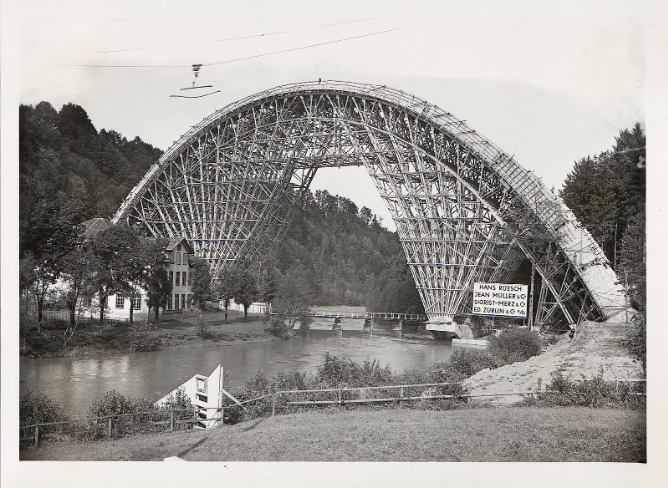
\includegraphics[width=0.75\linewidth]{images/infrastrukturgeschichte_bruecke.png}
\end{center}

\subsection{Was braucht es für funktionierenden Flugverkehr?}

Die Vorlesung zeigt am Beispiel des Flugverkehrs,
dass Technik nie isoliert funktioniert.

Ein Flugzeug allein reicht nicht,
damit Flugverkehr möglich wird.

Notwendig ist ein grosses Netz
aus technischen,
sozialen,
ökonomischen
und politischen Voraussetzungen.

Für funktionierenden Flugverkehr braucht es unter anderem:

\begin{itemize}
\item Orte zum Starten und Landen
\item technische Systeme zur Navigation und Kommunikation
\item Energie- und Treibstoffversorgung
\item Menschen zur Steuerung, Wartung und Koordination
\item Ausbildungs- und Wissenssysteme
\item Verwaltung, Regeln und internationale Abkommen
\item Sicherheits- und Kontrollsysteme
\item digitale Systeme zur Buchung und Organisation
\item globale Liefer- und Wartungsketten
\item Wetter-, Karten- und Informationssysteme
\item Kapital und wirtschaftliche Organisation
\item staatliche und internationale Institutionen
\item Verkehrsanbindungen zum Flughafen
\item Vertrauen in das Funktionieren aller Teilsysteme
\item Passagiere
\end{itemize}

Flugverkehr zeigt daher exemplarisch,
dass moderne Technik
auf Infrastrukturen angewiesen ist.

Technische Systeme funktionieren nur,
wenn viele weitere Systeme
gleichzeitig funktionieren.

\subsection{Strukturelle Bedingungen von Infrastruktur}

Infrastrukturen beruhen auf mehreren
strukturellen Bedingungen.

Erstens funktionieren sie als Netzwerke.

Technik ist Teil eines grösseren Netzes
aus Orten,
Menschen,
Energie,
Wissen
und Kommunikation.

Zweitens benötigen Infrastrukturen Koordination.

Unterschiedliche Akteure,
Institutionen
und technische Systeme
müssen aufeinander abgestimmt werden.

Drittens brauchen Infrastrukturen Standardisierung.

Gemeinsame Regeln,
Normen
und Verfahren
machen Anschlussfähigkeit
überhaupt erst möglich.

Ohne Standardisierung
könnten technische Systeme
nicht dauerhaft,
räumlich übergreifend
und gesellschaftlich verlässlich funktionieren.

\subsection{Infrastruktur als Teil „moderner“ Kulturen}

Infrastrukturen sind kein ausschliesslich modernes Phänomen.

Bereits alte Gesellschaften
bauten technische Systeme,
um Räume zu erschliessen,
Macht auszuüben
und Versorgung zu sichern.

Beispiele dafür sind:

\begin{itemize}
\item der chinesische Kaiserkanal
\item antike Wasserleitungen
\item das römische Strassensystem
\item das Strassensystem der Inka
\end{itemize}

Der chinesische Kaiserkanal
erschloss die Peripherie
mit dem Zentrum.

Das Strassennetz der Inka
erstreckte sich über den Westen Südamerikas
und ermöglichte die administrative Erschliessung
des Imperiums.

Wasserleitungen in Petra
machten einen Ort in der Wüste
überhaupt erst zu einem Macht-
und Wirtschaftszentrum.

Infrastrukturen sind daher
immer auch Mittel,
um Territorien nutzbar,
regierbar
und symbolisch bedeutungsvoll zu machen.

\begin{center}
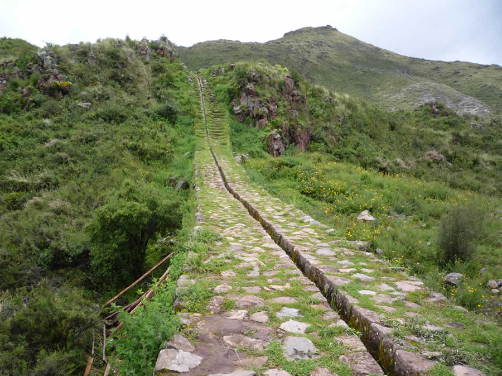
\includegraphics[width=0.85\linewidth]{images/infrastruktur_alte_kulturen.png}
\end{center}

\subsection{Infrastruktur und Modernität}

Modernität ist keine objektive Eigenschaft,
sondern eine Zuschreibung.

Infrastrukturen gelten häufig
als Zeichen von Modernität.

Sie zeigen,
dass gesellschaftliches Zusammenleben
organisiert,
geplant
und technisch unterstützt wird.

Gleichzeitig sollen Infrastrukturen
Modernität auch demonstrieren.

Grosse Brücken,
Kanäle,
Eisenbahnen,
Flughäfen
oder digitale Netze
können als Beweise technischer,
staatlicher
oder wirtschaftlicher Leistungsfähigkeit auftreten.

Infrastrukturen demonstrieren dadurch
auch Überlegenheit.

Sie zeigen,
wer planen,
bauen,
verbinden
und kontrollieren kann.

\subsection{Infrastruktur und Macht}

Infrastrukturen stehen in engem Zusammenhang
mit Macht.

Sie erschliessen und durchdringen Raum.

Strassen,
Kanäle
und Wegesysteme
machen Territorien zugänglich,
begehbar
und administrierbar.

Infrastrukturen können Machtzentren
überhaupt erst hervorbringen.

Aquädukte,
Wasserleitungen
oder Verkehrswege
machen manche Orte
erst zu Herrschafts-
und Handelszentren.

Zugleich vernetzen Infrastrukturen
Machtzentren mit Peripherien.

Sie verbinden administrative,
religiöse
und militärische Zentren
mit entfernten Regionen.

Dadurch ermöglichen sie staatliche Kohärenz
über grosse Räume hinweg.

Infrastrukturen sind auch Kommunikationssysteme.

Strassen,
Kanäle
und Wege dienen nicht nur dem Transport,
sondern auch der Übermittlung von Nachrichten,
Befehlen
und Informationen.

Sie ermöglichen Steuererhebung,
Truppenbewegung,
Versorgung
und damit die praktische Durchsetzung
politischer Ordnung.

\subsection{Kafka und die Chinesische Mauer}

Die Vorlesung bezieht sich auf Franz Kafkas Text
\emph{Beim Bau der Chinesischen Mauer} von 1917.

Darin wird die Chinesische Mauer
nicht nur als Schutzbauwerk betrachtet,
sondern als Projekt,
das über Jahrzehnte und Jahrhunderte
Arbeiterinnen und Arbeiter
aus dem ganzen Reich zusammenführt.

Die Mauer soll vor den „Nordvölkern“ schützen.

In weiten Teilen des Reiches,
etwa im Süden,
sind diese Nordvölker jedoch gar nicht bekannt.

Sie stellen dort keine unmittelbare Bedrohung dar.

Als Feind-
und Bedrohungsbild entstehen sie
erst durch das Bauprojekt selbst.

Kafka zeigt damit,
dass Infrastruktur nicht nur
auf bestehende politische Ordnung reagiert.

Sie bringt politische Ordnung
auch hervor.

Der Bau der Mauer beweist
der peripheren Bevölkerung,
dass es einen Kaiser,
ein Kaiserreich,
eine Dynastie
und damit ein chinesisches Reich gibt.

Infrastruktur stiftet also Zugehörigkeit,
auch dort,
wo die Machtzentrale
im Alltag kaum erfahrbar ist.

\subsection{Infrastruktur und Territorium}

Am Beispiel der Chinesischen Mauer wird sichtbar,
dass Infrastruktur Territorium erst herstellt.

Ein Reich ist nicht einfach dadurch gegeben,
dass es auf einer Karte existiert.

Es muss praktisch,
symbolisch
und materiell erfahrbar gemacht werden.

Grossprojekte wie Mauern,
Kanäle,
Strassen
oder Eisenbahnen
verbinden entfernte Regionen
mit einem politischen Zentrum.

Sie machen Macht sichtbar.

Sie schaffen Orientierung,
Zugehörigkeit
und Kontrollmöglichkeiten.

Territorium ist daher nicht nur Fläche.

Territorium entsteht durch Infrastrukturen,
die Raum erschliessen,
ordnen
und in politische Herrschaft übersetzen.

\subsection{Kongokonferenz in Berlin 1884}

Ein weiteres Beispiel für den Zusammenhang
von Infrastruktur,
Territorium
und Macht
ist die Kongokonferenz in Berlin 1884.

Dort trafen sich europäische Mächte
unter der Leitung von Otto von Bismarck.

Ziel war es,
Regeln für die koloniale Expansion in Afrika festzulegen
und Konflikte zwischen europäischen Staaten zu vermeiden.

Ein zentrales Prinzip war
die sogenannte „effektive Okkupation“.

Territoriale Ansprüche galten nur dann,
wenn tatsächliche Kontrolle ausgeübt wurde.

Dies beschleunigte den kolonialen Wettbewerb
um Afrika,
den sogenannten \emph{Scramble for Africa}.

Infrastruktur wurde dadurch
zum Beweis staatlicher Herrschaft.

Wer Strassen,
Bahnlinien,
Telegrafie
und Verwaltungszentren errichtete,
konnte territoriale Ansprüche legitimieren.

\begin{center}
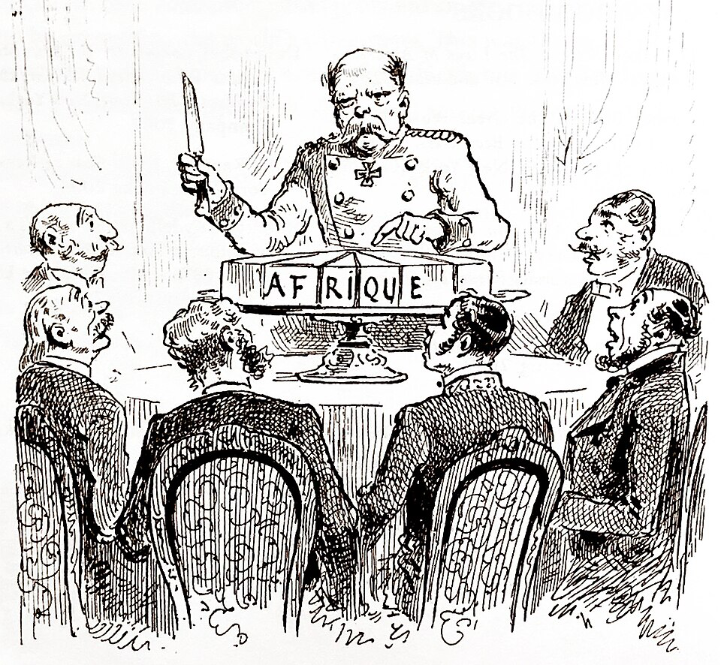
\includegraphics[width=0.75\linewidth]{images/kongokonferenz_berlin_1884.png}
\end{center}

\subsection{Infrastruktur als imperiale Strategie}

Koloniale Infrastruktur diente selten
primär der lokalen Entwicklung.

Zwar wurde Kolonialismus häufig damit gerechtfertigt,
dass koloniale Gebiete zivilisiert
und modern gemacht würden.

Tatsächlich wurde Infrastruktur jedoch vor allem
für imperiale Zwecke aufgebaut.

Dazu gehörten:

\begin{itemize}
\item militärische Mobilität
\item Rohstoffexport
\item Steuererhebung
\item Kommunikation zwischen Küste und Inland
\item Sichtbarmachung staatlicher Macht
\end{itemize}

Wer über Infrastruktur nachdenkt,
muss daher fragen:

\begin{itemize}
\item Wer baut?
\item Wer finanziert?
\item Wer betreibt?
\item Wer nutzt?
\item Wem nützt die Infrastruktur?
\end{itemize}

Infrastruktur war und ist nicht bloss Technik.

Sie ist ein Mittel,
Territorien überhaupt erst
als regierbare Räume hervorzubringen.

\subsection{Postkoloniale Infrastruktur}

Auch nach der Unabhängigkeit
einst kolonisierter Staaten
blieben Infrastrukturen politisch bedeutsam.

Sie konnten weiterhin eine Möglichkeit
zur Einflussnahme
für ehemalige Kolonialmächte darstellen.

Dies verweist auf postkoloniale Machtverhältnisse.

Ein Beispiel ist die Kenya and Uganda Railroad.

Sie führte vom Landesinnern
zu den Handelsstädten an der Küste.

Solche Infrastrukturen waren häufig
auf koloniale Interessen ausgerichtet.

Sie verbanden Rohstoffgebiete
mit Häfen,
Verwaltungszentren
und imperialen Handelswegen.

Für lokale Bevölkerungen bedeuteten sie nicht unbedingt
eine gleichmässige Erschliessung
oder Verbesserung der Lebensbedingungen.

Vielmehr ordneten sie Räume
nach kolonialen Interessen.

\begin{center}
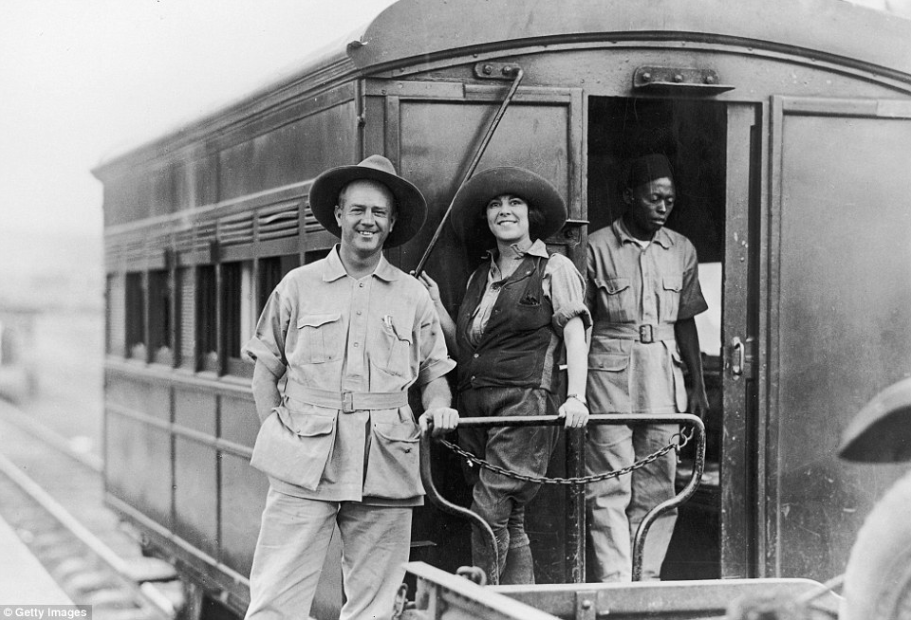
\includegraphics[width=0.75\linewidth]{images/kenya_uganda_railroad.png}
\end{center}

\subsection{Normativität und Alltag}

Im Verlauf des 20. Jahrhunderts
wurden immer mehr Menschen
auf infrastrukturelle Leistungen angewiesen.

Sie kamen regelmässig
mit Infrastrukturen in Kontakt.

Dazu gehören unter anderem:

\begin{itemize}
\item öffentlicher Verkehr
\item Spitäler
\item Stromversorgung
\item Kommunikation
\item Wasser
\item Internet
\end{itemize}

Infrastrukturen organisieren nicht nur Versorgung
und Mobilität.

Sie prägen auch,
wie Menschen leben,
handeln
und denken.

Sie legen fest,
was als normal
oder selbstverständlich erscheint.

Das Stromnetz erzeugt zum Beispiel
die Erwartung dauerhafter Verfügbarkeit
von Licht,
Arbeit
und elektrischen Geräten.

Autogerechte Städte machen das Auto
zur dominanten Mobilitätsform
und prägen das Erscheinungsbild
von Städten und Landschaften.

Infrastrukturen lenken Verhalten.

Sie machen bestimmte Handlungen einfach
und andere schwierig.

Ihre normative Kraft fällt meist erst dann auf,
wenn sie ausfallen.

Wenn Strom,
Wasser,
Internet
oder Verkehrssysteme nicht funktionieren,
wird sichtbar,
wie abhängig der Alltag
von Infrastruktur ist.

\subsection{Infrastruktur als materialisierte gesellschaftliche Ordnung}

Seit spätestens der zweiten Hälfte
des 20. Jahrhunderts
ist Infrastruktur materialisierte
gesellschaftliche Ordnung.

Sie organisiert gesellschaftliches Zusammenleben
und prägt individuellen Alltag.

Infrastrukturen sind daher nicht neutral.

Sie enthalten Vorstellungen davon,
wie Menschen leben sollen,
wie Räume genutzt werden sollen
und welche Formen von Mobilität,
Kommunikation
oder Versorgung selbstverständlich sind.

Das Beispiel der tiefen Brücken
von Robert Moses auf Long Island zeigt dies besonders deutlich.

Die Brücken waren zu niedrig
für Fahrzeuge des öffentlichen Verkehrs.

Dadurch wurde der Zugang zu bestimmten Parks
faktisch Menschen mit PKW vorbehalten.

Infrastruktur konnte somit soziale Ungleichheit
und Ausschluss materiell festschreiben.

Technische Gestaltung
wurde zu sozialer Ordnung.

\subsection{Worauf baut unsere digitale Welt?}

Die Vorlesung fragt abschliessend,
worauf die digitale Welt eigentlich baut.

Digitale Räume erscheinen häufig immateriell
oder virtuell.

Tatsächlich beruhen sie jedoch
auf umfangreichen materiellen Infrastrukturen.

Dazu gehören:

\begin{itemize}
\item Rechenzentren
\item Glasfasernetze
\item Unterseekabel
\item Stromversorgung
\item Kühlung
\item Plattformarchitekturen
\item Datenprotokolle
\item seltene Erden
\item Arbeitskräfte
\item Lieferketten
\end{itemize}

Auch die digitale Welt hat daher
eine territoriale Grundlage.

Sie benötigt Orte,
Energie,
Rohstoffe,
Gebäude,
Netzwerke
und politische Rahmenbedingungen.

Wichtige Fragen lauten:

\begin{itemize}
\item Was ist die Infrastruktur des Digitalen?
\item Wer betreibt sie?
\item Wo befindet sie sich?
\item Wer zahlt?
\item Wer baut sie auf?
\item Wer nutzt sie?
\end{itemize}

\subsection{Virtualität und Territorium}

Digitale Infrastrukturen sind eng
mit anderen Infrastrukturen verbunden.

Kommunikation,
Militär,
Mobilität,
Industrie,
Finanzmarkt,
Logistik
und Bildung
sind zunehmend auf digitale Systeme angewiesen.

Gleichzeitig bauen digitale Infrastrukturen
auf älteren Infrastrukturen auf.

Schon immer wurden Infrastrukturen
auf andere Infrastrukturen aufgebaut.

Kommunikation und Transport
waren beispielsweise historisch eng verbunden.

Auch Rechenzentren
sind nicht einfach virtuelle Räume.

Sie brauchen Strom,
Kühlung,
Gebäude,
Sicherheit,
Netzanbindung
und politische Regulierung.

Die digitale Infrastruktur wirkt daher territorial,
ähnlich wie frühere Infrastrukturen
wie das Strassennetz der Inka,
der chinesische Kaiserkanal,
Eisenbahnen
oder Brücken.

Sie ordnet Räume,
schafft Abhängigkeiten,
ermöglicht Kontrolle
und verbindet Zentren mit Peripherien.

\begin{center}
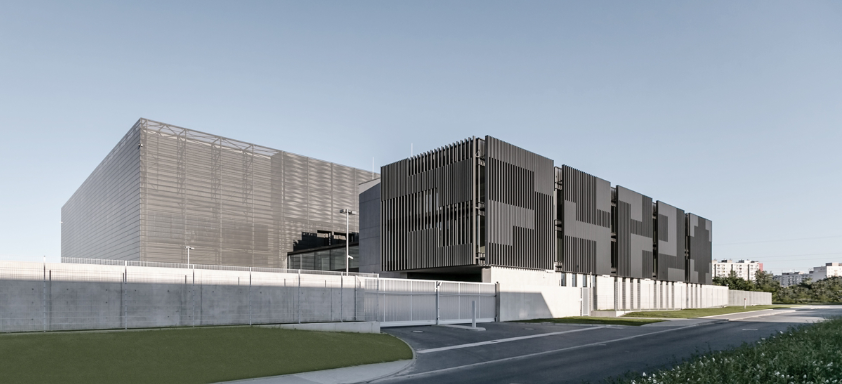
\includegraphics[width=0.75\linewidth]{images/data_center_poznan.png}
\end{center}

\subsection{Zentrale Erkenntnisse}

Die Vorlesung zeigt,
dass Infrastrukturen weit mehr leisten
als technische Versorgung.

Sie erschliessen Räume,
organisieren Gesellschaft,
stabilisieren Macht
und prägen Alltag.

Zentrale Erkenntnisse sind:

\begin{itemize}
\item Infrastrukturen funktionieren als Netzwerke aus Technik, Menschen, Energie, Wissen und Institutionen.
\item Sie benötigen Koordination und Standardisierung.
\item Infrastrukturprojekte dienten historisch der Raumerschliessung, Machtausübung und Demonstration von Modernität.
\item Infrastrukturen machen Territorien zugänglich, administrierbar und regierbar.
\item Koloniale Infrastruktur diente häufig imperialen Interessen statt lokaler Entwicklung.
\item Infrastrukturen prägen Alltag, Normalität und Verhalten.
\item Digitale Welten beruhen auf materiellen und territorialen Infrastrukturen.
\end{itemize}

Die zentrale These lautet:

Infrastruktur ist nicht bloss technische Grundlage
gesellschaftlichen Lebens.

Sie ist materialisierte Ordnung.

Sie schafft Räume,
regelt Zugang,
organisiert Macht
und macht Gesellschaften
in bestimmter Weise handlungsfähig.

Wer Infrastrukturen baut,
kontrolliert oder nutzt,
gestaltet daher nicht nur Technik,
sondern auch Territorium,
Alltag
und gesellschaftliche Möglichkeiten.
